
\section{Контрольные переменные, чтобы измежать смещения}

% \begin{frame}{Мотивационный пример 1 }
%   Thompson estimator 
%   https://link.springer.com/article/10.1023/A:1020363010465
% \end{frame}

\subsection{Примеры}

\begin{frame}{Пример: эффект от обучения на результаты по математике \parencite{barnard2003principal}}
% В целом, это плохой пример блокинга. Надо еще поискать. Тут не вполне блокинг в конце концов и цифры так себе
    \begin{itemize}
        \item Абитуриентам из бедных семей случайным образом предлагалась грант на обучение в частной школе
        \item Предполагалось выдавать грант случайным образом, но
        \begin{itemize}
            \item Детям из сильных школ давали грант с большей вероятностью
        \end{itemize}
        \item Выполнено ли $(X, Y_1, Y_0) \perp T$?
   \end{itemize}
\end{frame}

\begin{frame}{Схема}
\end{frame}


\begin{frame}{Что если оценить вот так?}

\begin{gather*}
\text{ATE} = \frac{N_H}{N} \left(\frac{1}{N_{TH}}\sum_{T=1, S=H} Y - \frac{1}{N_{CH}}\sum_{T=0,S=H} Y \right)+ \\
\frac{N_L}{N} \left(\frac{1}{N_{TL}}\sum_{T=1, S=L} Y - \frac{1}{N_{CL}}\sum_{T=0,S=L} Y \right)
\end{gather*}

\end{frame}


\begin{frame}{Проверка баланса ковариатов}
    \begin{figure}
     \centering
     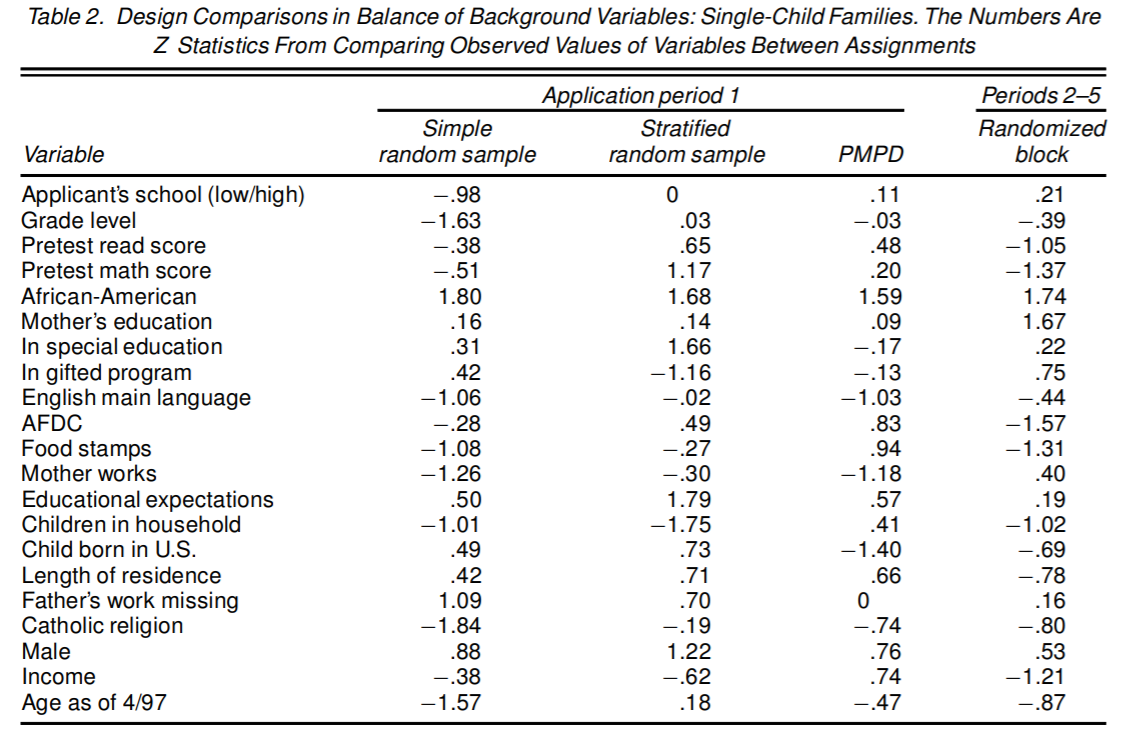
\includegraphics[width=\textwidth]{Images/Matching1.png}
\end{figure}
\end{frame}

\begin{frame}{Пример 2: Долгосрочный эффект от R\&D  \parencite{schweiger2018long}}
\begin{figure}
    \centering
    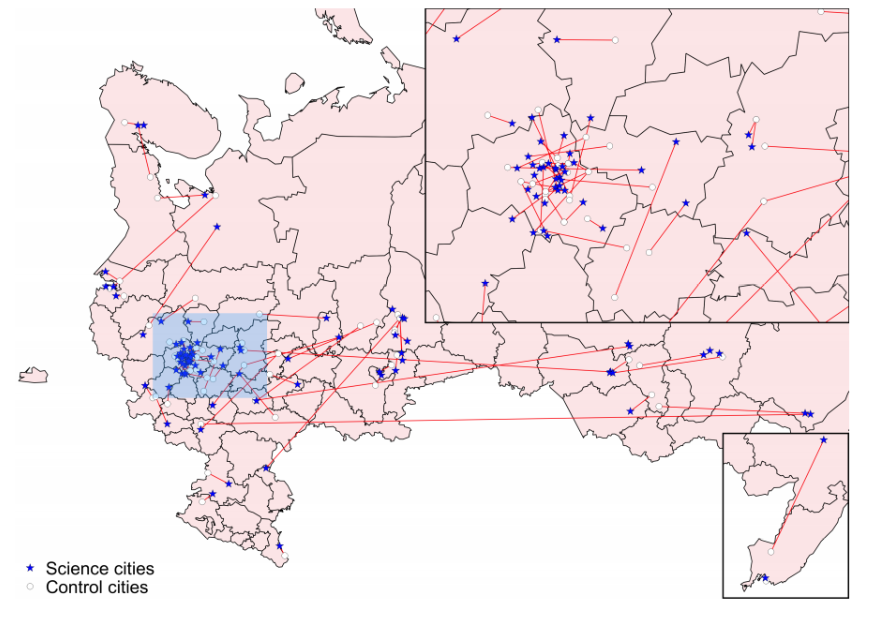
\includegraphics[width=\textwidth]{Images/Naukograds.png}
\end{figure}
\end{frame}

\subsection{Confounders}

\begin{frame}{Проблема в Confounders}
\begin{itemize}
   \item Covariates -- X, коррелирующие с Y
   \item Confounders -- X, коррелирующие с Y и с T
   % \item Какое решение проблемы вы уже знаете?
\end{itemize}

Схема

\end{frame} 

% здесь нужна секция про conrtol просто приямым образом и что со схемой делает

\begin{frame}{Иллюстрация 1}
\begin{table}[]
\begin{tabular}{l|l|l||l}
&$Y_1$ & $Y_0$ & X \\
\hline
Пациент 1 & - & 37.8 & Из Европы \\
Пациент 2 & - & 37.6 & Из Европы  \\
Пациент 3 & - & 40 & Из Азии  \\
Пациент 4 & 36.6 & - & Из Европы  \\
Пациент 5 &38   & - &  Из Азии \\
Пациент 6 &39.2 & - & Из Азии
\end{tabular}
\end{table}

В чем проблема и что можно сделать?
\begin{itemize}[<+->]
        \item Нет баланса по X!
        \item Что с $T_i \perp (Y(1)_i, Y(0)_i, X_i)$ ?
        \item Мы можем посчитать эффект отдельно для каждой подгруппы
\end{itemize}
\end{frame} 


\begin{frame}{Иллюстрация 2}
\begin{table}[]
\begin{tabular}{l|l|l||l}
&$Y_1$ & $Y_0$ & X \\
\hline
Пациент 1 & - & 37.8 & Эксперимент в 2019 P = 0.33 \\
Пациент 2 & - & 37.6 & Эксперимент в 2019 P = 0.33 \\
Пациент 4 & 36.6 & - & Эксперимент в 2019 P = 0.33  \\
Пациент 3 & - & 40 & Эксперимент в 2020 P = 0.66 \\
Пациент 5 &38   & - &  Эксперимент в 2020 P = 0.66 \\
Пациент 6 &39.2 & - & Эксперимент в 2020 P = 0.66
\end{tabular}
\begin{itemize}
        \item В экспериментах разные P. По чему теперь нет баланса?
        \item Что с $T_i \perp (Y(1)_i, Y(0)_i, X_i)$ ?
        \item Для каждой группы отдельно выполнено?
\end{itemize}
\end{table}
\end{frame}

\begin{frame}{Иллюстрация 3}
\begin{table}[]
\begin{tabular}{l|l|l||l}
&$Y_1$ & $Y_0$ & X \\
\hline
Пациент 1 & - & 37.8 & Эксперимент в 2019 P = 0 \\
Пациент 2 & - & 37.6 & Эксперимент в 2019 P = 0 \\
Пациент 4 & - & 36.6 & Эксперимент в 2019 P = 0  \\
Пациент 3 & 40 & - & Эксперимент в 2020 P = 1 \\
Пациент 5 &38   & - &  Эксперимент в 2020 P = 1 \\
Пациент 6 &39.2 & - & Эксперимент в 2020 P =1
\end{tabular}
\begin{itemize}
        \item Можем что-то сделать?
\end{itemize}
\end{table}

\end{frame} 

\subsection{Предположение условной независимости}

\begin{frame}{Unconfoundedness\footcite[Раздел 3.2.1]{angrist2008mostly} и Overlap}
\begin{itemize}
   \item $T_i \perp (Y(1)_i, Y(0)_i, X_i)$ - идеальный эксперимент
   \item Вероятность попасть в тритмент-группу известна и одинакова для всех
   \item $T_i \perp (Y(1)_i, Y(0)_i) | X_i$ - unconfoundedness (CIA, conditional independence assumption). Если взять людей с одинаковыми харатеристиками, то факт, что они в такой-то группе, не зависит от потенциальных исходов
   \item $e(X_i)=E(D_i | X_i) \in (0,1) $ - overlap. Вероятность попадания в тритмент-группу зависит от характеристик и ненулевая для всех значений Х
\end{itemize}
\end{frame}

\begin{frame}{Итого:}
\begin{gather*}
\text{ATE} = \frac{N_H}{N} \left(\frac{1}{N_{TH}}\sum_{T=1, S=H} Y - \frac{1}{N_{CH}}\sum_{T=0,S=H} Y \right)+ \\
\frac{N_L}{N} \left(\frac{1}{N_{TL}}\sum_{T=1, S=L} Y - \frac{1}{N_{CL}}\sum_{T=0,S=L} Y \right)
\end{gather*}

\begin{itemize}
    \item Что не так, если не выполнено unconfoundedness?
    \item Что не так, если не выполнен overlap?
    \item Как получить ATT?
    \item Что делать, если X принимает слишком много разных значений?
\end{itemize}
\end{frame}

% \begin{frame}{Balancing score}
% Propscore, который ухуджает
% \end{frame}
